\documentclass[11pt,titlepage]{article}

%Laenderspezifische Einstellungen bzgl. Rechtschreibung, Sonderzeichen und Kodierung
\usepackage[utf8]{inputenc}
\usepackage[english]{babel}
\usepackage[T1]{fontenc}
\usepackage{titlesec}
\usepackage{graphicx}
%\usepackage{subcaption}

\usepackage{listings}
\usepackage{color}
\usepackage{courier}
\definecolor{light-gray}{gray}{0.85}
\lstset{
language=C++,
numbers=left,
breaklines=true,
backgroundcolor=\color{light-gray},
tabsize=2,
basicstyle=\footnotesize\ttfamily,
frame=single,
inputencoding=utf8,
extendedchars=true,
showstringspaces=false,
literate =
	{ä}{{\"a}}1
	{ö}{{\"o}}1
	{ü}{{\"u}}1
	{Ä}{{\"A}}1
	{Ö}{{\"O}}1
	{Ü}{{\"U}}1
	{ß}{{\ss}}1
	{ₙ}{{$_n$}}1
}

\def\ContinueLineNumber{\lstset{firstnumber=last}}
\def\StartLineAt#1{\lstset{firstnumber=#1}}		%\StartLineAt{xxx}	

\usepackage[
	a4paper,
	top = 2cm,
	bottom = 2 cm,
	left = 2cm,
	right = 2cm,
	headheight = 15pt,
	includeheadfoot
	]{geometry}
\usepackage{fancyhdr}
\usepackage{amssymb}
\usepackage{amsmath}
\usepackage[english]{varioref}
\usepackage{hyperref}

\fancypagestyle{fancy}{
	\fancyhead[R]{Page \thepage}
	\fancyhead[L]{\leftmark}
	\renewcommand{\headrulewidth}{1.25pt}

	\fancyfoot[L]{\tiny{Programming 2 - Assignment 3, created: \today}}
	\fancyfoot[R]{\tiny{ Felix Dreßler (k12105003)}}
	\cfoot{}
	\renewcommand{\footrulewidth}{1.25pt}
}

\setlength{\headsep}{10mm}
\setlength{\footskip}{10mm}

\setlength{\parindent}{0mm}
\setlength{\parskip}{1.1ex plus0.25ex minus0.25ex}
\setlength{\tabcolsep}{0.2cm} % for the horizontal padding

\pagestyle{fancy}

\title{Programming 2 - Assignment 3}
\author{Felix Dreßler (k12105003)\\ email \href{mailto:FelixDressler01@gmail.com}{FelixDressler01@gmail.com}}
\date{\today} %Erstellungsdatum

\begin{document}
\maketitle
	\section{The Program}
	

		\subsection{The Program - Polygon}
			\subsubsection{Polygon.h}
				\lstinputlisting[]{Assignment3/Project1/Polygon.h}
				
			\subsubsection{Polygon.cpp}
				\lstinputlisting[]{Assignment3/Project1/Polygon.cpp}
		
		\subsection{The Program - Picture}
			\subsubsection{Picture.h}
				\lstinputlisting[]{Assignment3/Project1/Picture.h}
			
			\subsubsection{Picture.cpp}
				\lstinputlisting[]{Assignment3/Project1/Picture.cpp}
		
		\subsection{The Program - Linked Lists}
			\subsubsection{LinkedListArr.h}
				\lstinputlisting[]{Assignment3/Project1/LinkedList.h}
			
			\subsubsection{LinkedListArr.cpp}
				\lstinputlisting[]{Assignment3/Project1/LinkedList.cpp}
			
			\subsubsection{LinkedListPointer.h}
				\lstinputlisting[]{Assignment3/Project1/LinkedListPointer.h}
				
			\subsubsection{LinkedListPointer.cpp}
				\lstinputlisting[]{Assignment3/Project1/LinkedListPointer.cpp}
				
	\section{Problems}
	This section will briefly discuss the Problems that have occurred during programming.
		\subsection{warnings}
		In the \emph{resize} method, line 283 of the \emph{DistPoly.cpp} this warning is displayed:
		
			%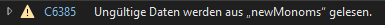
\includegraphics[scale=1.5]{Documentation/warning-line297.png}
		
	
\end{document}